\documentclass[a4paper, 10pt, dvipdfmx]{jlreq}

\usepackage{amsmath,amsfonts,amssymb}
\usepackage{bm}
\usepackage{mathtools}
\usepackage{siunitx}
\usepackage[dvipdfmx]{graphicx}
\usepackage[dvipdfmx]{color}
\usepackage[dvipdfmx, colorlinks=true, allcolors=blue]{hyperref}
\usepackage{listings, jlisting}
\usepackage{tikz}
\usepackage{physics}
\usepackage{url}

\Urlmuskip=0mu plus 10mu
\allowdisplaybreaks[4]
\frenchspacing
\definecolor{OliveGreen}{rgb}{0.0,0.6,0.0}
\definecolor{Orenge}{rgb}{0.89,0.55,0}
\definecolor{SkyBlue}{rgb}{0.28, 0.28, 0.95}
\lstset{
  language={c++},
  basicstyle={\ttfamily},
  identifierstyle={\small},
  ndkeywordstyle={\small},
  frame=single,
  breaklines=true,
  numbers=left,
  xrightmargin=0zw,
  xleftmargin=3zw,
  numberstyle={\scriptsize},
  lineskip=-0.9ex,
  keywordstyle={\small\bfseries\color{SkyBlue}},  
  commentstyle={\color{OliveGreen}}, 
  stringstyle={\small\ttfamily\color{Orenge}}    
}

\begin{document}

\title{2010年度 大問4}
\author{hari64boli64 (hari64boli64@gmail.com)}
\date{\today}
\maketitle

\section{問題}

算数

\section{解答}

\subsection*{(1)}

\begin{align*}
  w_1(t_{i+1})=2\min(1-\alpha,\alpha) \\
  w_2(t_{i+1})=\max(0,1-2\alpha)      \\
  w_3(t_{i+1})=\max(0,2\alpha-1)      \\
\end{align*}

\subsection*{(2)}

\begin{center}
  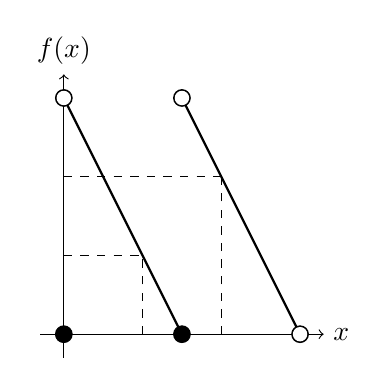
\begin{tikzpicture}[scale=3]
    \draw[->] (-0.1,0) -- (1.1,0) node[right] {$x$};
    \draw[->] (0,-0.1) -- (0,1.1) node[above] {$f(x)$};
    \draw[dashed] (1/3,0) -- (1/3,1/3);
    \draw[dashed] (0,1/3) -- (1/3,1/3);
    \draw[dashed] (0,2/3) -- (2/3,2/3);
    \draw[dashed] (2/3,0) -- (2/3,2/3);
    \draw[thick] (0,1) -- (1/2,0);
    \draw[thick] (1/2,1) -- (1,0);
    \filldraw[black] (0,0) circle (1pt);
    \filldraw[black] (1/2,0) circle (1pt);
    \filldraw[black] (0,1) circle (1pt);
    \filldraw[white] (0,1) circle (0.8pt);
    \filldraw[black] (1/2,1) circle (1pt);
    \filldraw[white] (1/2,1) circle (0.8pt);
    \filldraw[black] (1,0) circle (1pt);
    \filldraw[white] (1,0) circle (0.8pt);
  \end{tikzpicture}
\end{center}

\subsection*{(3)}

ヒントを示すのは、面倒だが自明。
ヒントを使うのは、繰り返せば自明。

\end{document}
